% -*- coding: utf-8 -*-

% TODO:
% CUDA programmeringsmodel, device, host, recursion, function pointers, etc.
% CUDA hukommelsesmodel, bank conflicts, etc
% Paracuda argumentation for interface (makroer)
% Paracuda hjælpefunktioner
% Paracuda implementation
% Dokumentation af implementerede algoritmer oven på biblioteket
% Korrekthedstests - DONE
% Benchmarks af vores og andres:
%   host single thread vs vores device multi thread
%   nvidias scan vs vores scan
%   host single thread vs vores device multi thread sortering
% Konklusion:
%   anvendelighed - for alle eller kun dedikerede performance folk?
%   cuda - er det umagen værd?
%   hastighedsforøgelse vs arbejdsbyrde

\documentclass[11pt,oneside,a4paper]{article}
\usepackage[danish]{babel}
\usepackage[utf8]{inputenc}
\usepackage{latexsym}
\usepackage{listings}
\usepackage{url}
\usepackage{ulem}
\usepackage{amsmath, amssymb, amsthm}
\newcommand{\modelDesc}[4]{
\emph{#1:}\\
\texttt{Input:}
\begin{description}
#2
\end{description}
\texttt{Beskrivelse:}\\
#3\\
\texttt{Eksempel:}\\
#4\\
}
\usepackage{graphicx}
\newcommand{\sourcecode}[3]{
\subsection{#3}
\label{#2}
{\scriptsize
\lstinputlisting[breaklines=true]{../sdk/projects/paracuda/#1}
}
}
\newcommand{\hide}[1]{}
\title{Parallel-vector-modellen på GP-GPU via CUDA}
\author{Joakim Ahnfelt-Rønne \and Mikkel Kjær Jensen}
\date{17. april 2009}
\begin{document}
\maketitle
\abstract{
Vi har undersøgt hvorvidt \cite{ble} Vektor-Scan for parallelisme er realiserbar
på grafikkort via CUDA, NVIDIAs standard for GP-GPU-beregninger.
Vi har implementeret et bibliotek der gør det muligt at bruge modellen til at
programmere på grafikkort uden at skulle kende til CUDA. Denne er
imidlertid for langsom til at være brugbar i praksis.
Vi har undersøgt hvorvidt det ville gøre modellen brugbar hvis man erstattede
vores scan-primitiv med NVIDIAs egen implementation, som er betydeligt hurtigere.
Vi argumenterer for at modellen ikke er brugbar selv med denne implementation.
Vi beskriver desuden hvad der gør NVIDIAs implementation hurtigere end vores.}

\tableofcontents

% -*- coding: utf-8 -*-

% NOTER TIL DETTE AFSNIT:
% - Motivation
%   - Hvorfor CUDA? (meget udbredt, mulige masseproduktionsfordele).
%   - Hvorfor vector/scan? (nævn evt. at det kunne være vejen til
%     at impelmentere en backend for det der vector/scan sprog,
%     eller i hvert fald en undersøgelse om det kunne betale sig).
% - Mål
%   - Er vector/scan-modellen realistisk på CUDA?
%   - Hvor arbejdskrævende er det at benytte CUDA?
%   - Hvad skal man vide for at benytte CUDA?
%   - Hvordan optimerer man på CUDA?
% - Fokus
% - Læringsmål

\section{Introduktion}
I de sidste par år er man ved at have nået en hardwaremæssig grænse for hvor
hurtigt sekventiele programmer kan afvikles, og man er derfor begyndt at fokusere på at eksekvere programmerne
parallelt. Dette har allerede længe været tilfældet for GPU'er (Graphical Prosessing Units), som typisk kommer med mange kerner, og som samtidigt ligger i en overskuelig prisklasse. Det er derfor interessant 
at undersøge hvordan man bedst udnytter sådanne processorer til generelle algoritmer. 

Der findes algoritmer der er åbentlyst paralleliserbare (map), men også mindre åbentlyse algoritmer, som at 
summere værdierne i en vektor, kan gøres effektivt parallelt. Scan er generalisering af dette, der anvender en associativ operator på elementerne i vektoren, og efterlader præfix-summen op til hvert element på elementets position. En måde at implementere disse på er vha. vektor-scan modellen, som tillader skabelsen af mange primitiver der kan bruges til at udvikle generelle algoritmer, samtidigt med at de er designet til at kunne eksekveres i et paralelt miljø - som f.eks. NVIDIAs CUDA platform.

\subsection{Mål}

Vi vil i dette projekt undersøge om det kan betale sig at implementere vector-scan modellen på CUDA, med det formål at demonstrere en implementation af Scan på NVIDIAs CUDA platform. Vi vil i dette projekt desuden gøre det til vores mål at lære at programmere på CUDA platformen, samt at forstå scan-vector modellen, og videregive de erfaringer vi har gjort os - med særlig fokus på optimering.

For at give en kvantitativ indikator af hvor godt vores projekt har lykkedes, vil vi sammenligne vores egne implementationer med CUDA's implementation af scan, samt en sekventiel version af algoritmen.\\

% -*- coding: utf-8 -*-
% NOTER TIL DETTE AFSNIT:
% - Skriv om Cuda:
%* Hvad er det
%* Hvem har lavet det
%* hvad skal man bemærke sig ved det

\section{CUDA}
\label{CUDA}
\subsection{Introduktion}

CUDA, som står for ``Compute Unified Device Architecture'', er en arkitektur udviklet af grafikkort producenten NVIDIA, der tillader programmører skrive generel purpose programmer der kan eksekveres på et NVIDIA grafikkort. Ideen er at udnytte grafikkortenes mange kerner til at udføre mange paralle udregninger. Alle programmer der skal eksekveres på CUDA skal skrives i ``C for CUDA'', som er en modificeret version af C, der indeholder de nødvendige datastrukturer og funktioner til at man kan skrive en funktion, en såkaldt kernel, der eksekveres parallelt på grafikkortet. Udvidelserne kan placeres i 3 primære kategorier:

\begin{description}
\item[Host:] Funktioner der kan eksekveres på CPU'en og som kan tilgå GPU'en/GPU'erne.
\item[Device:] Funktioner der kun kan eksekveres på GPU'en, og som kun har relevans for kortet
\item[Fælles:] Indbyggede datastrukturer samt en delmængde af C's bibliotek, der både kan køre på CPU'en såvel som GPU'en.
\end{description}


\subsection{Blokke og tråde}

Et vigtigt begreb i CUDA er blokke og tråde. For at udnytte grafikkortets parallelle potentiale optimalt, bliver alle udregningerne på GPU'en udført i tråde. Videre er disse tråde inddelt i blokke for nem håndtering. Hver blok kan i CUDA 2.1 indeholde op til 512 tråde og kan inden for blokken dele delt hukommelse (se \ref{CudaHukom}), samt synkronisere deres eksekvering. Den maksimale størrelse på en blok udgør derfor en naturlig størrelse at splitte større parallelle problemer op i, hvis udregningerne afhænger af tidligere resultater - se også \ref{CudaHukom}. Blokke der er lige store bliver i så høj grad som muligt eksekveret parallelt, hvilket betyder at det, alt efter situationen, kan betale sig at allokere tråde i multipla af 512 (eller hvor meget der vælges at bruge pr. blok), og så sørge for at de ekstra tråde ikke foretager sig noget.

Modsat på CPU'en, vil tråde på GPU'en eksekvere hele kernelen. Hvis en blok støder på conditional statements (\texttt{if}, \texttt{if-else}, \texttt{switch}, etc.) vil alle veje igennem kernelen eksekveres - de tråde som ikke opfylder betingelsen bliver blot deaktiveret i den del af koden \cite{cuda-guide}. Det er derfor tilrådeligt at have så få conditional statements i koden som muligt, da alle branches skal gennemgås.

\subsection{Kernel}
Når en kernel køres, vil alle dens tråde arbejde på samme inddata, så den eneste måde at differentiere tråde på er vha. deres threadId og id'et på den blok de tilhører.

\subsection{Hukommelse}
\label{CudaHukom}
CUDA skelner mellem hukommelse der er tilgængelig fra CPU'en (``host memory'') og hukommelse der er tilgængelig fra GPU'en (``device memory''). Hvis man tilgår en forkert type hukommelse vil det enten resultere i segmentation faults eller udefineret data. Omkostningen ved at kopiere fra den ene til den anden er ikke ubetydeligt, og det kan derfor anbefales, at man prøver at undgå konstant at kopiere data frem og tilbage.

Når man skriver programmer på CUDA, er hukommelse noget af det vigtigste at optimere.

På GPU'en er de to vigtigste hukommelser den lille, men hurtige, delte hukommelse og den store, men langsomme globale hukommelse. For begge hukommelser tager det fire maskine cykler at skedulere at man vil gemme eller hente data - men for den globale hukommelse er der endvidere et overhead på 400-600 cykler hver gang det enten skal læses eller skrives. For at kunne udnytte CUDA ordentligt, er det derfor imperativt kun at tilgå den globale hukommelse så lidt som muligt, og derimod udnytte den delte hukommelse. Da denne hukommelse er lille og isoleret i hver blok, vil det, for algoritmer der skal arbejde på på store datamængder, være nødvendigt at finde en metode til at splitte algoritmen op i flere faser, og eventuelt til sidst lave en korrigering af data for at få et korrekt resultat.

Et problem der kan opstå når man bruger sekventiel hukommelse er bank conflicts. For at gøre hukommelses tilgangen i den delte hukommelse hurtigere, er den delte splittet op i flere lige store dele, kaldet banks, så hver bank kan tilgås af en tråd samtidigt. Hvis flere tråde prøver at tilgå den samme bank i hukommelsen, vil hardwaren være nød til at tilgå bank'en sekventielt. Et godt eksempel på at undgå dette bliver vist i implementeringen af Scan primitiven\footnote{Se \ref{ScanPrim}, s. \pageref{ScanPrim}} i \cite{gpu-scan}.

For videre information om CUDA henvises der til \cite{cuda-guide}.

% -*- coding: utf-8 -*-

% NOTER TIL DETTE AFSNIT:
% - Der er nogle relevante iagtagelser her som måske fortjæner sit eget afsnit.
% - Ellers flet det ind i introduktionen.

\section{Overvejelser}

\subsection{Tidspunkt for valg af operator}

I vores projekt valgte vi at starte med at implementere Scan, da den både var overkommelig at implementere, samtidigt med at den dannede fundament for mange andre algoritmer - som Split og Quicksort.

Som nævnt tidligere i rapporten så virker Scan med alle associative binære operatorer, der sammen med et
neutralt element danner en monoid. 
Derfor ville det være interessant at give brugeren af biblioteket muligheden at vælge, eller ligefrem implementere, den ønskede associative operator.

Et vigtigt spørgsmål, vi blev nød til at tage stilling til, var derfor på hvilket tidspunkt den nødvendige operator skulle vælges. Dette efterlader os med to valgmuligheder, enten på køretidspunktet eller overættelsestidspunktet:

\begin{itemize}
\item Muligheder på køretidspunktet:
\begin{itemize}
\item At generere "PTX" assembler kode og lade driveren oversætte denne til NVIDIA maskinkode. Dette kræver dog at vi bruger driver-api'et som ikke er tilgængeligt i emulatoren.
\item At skrive en fortolker der kører i trådene og generere kode til denne.
\end{itemize}

\item Muligheder på oversættelsestidpunktet:
\begin{itemize}
%\item At generere CUDA-kode og sammensætte den med et scan-skelet.
%\item At lade sproget for operatorer være CUDA og så generere CUDA-kode ved at sammensætte operatoren  med et scan-skelet.
\item At bruge makroer
\item At bruge klasser
\item At bruge templates
\end{itemize}
\end{itemize}

\subsubsection{Run Time}
Vi mente at PTX løsningen var urealistisk, da den ville krævede adgang
til et grafikkort under hele udviklingsforløbet, samt at vi skulle sætte os ind i assembler-sproget, hvilket ville tage alt for lang tid. Desuden ville det at skrive en oversætter være et større projekt i sig selv, og ændre fokus for projektet.

Ligeledes mente vi at det ville være både for perifert til vores opgave, samt for tidskrævende at designe vores eget domæne specifikke sprog og skrive en fortolker til denne.

Da CUDA ikke understøtter funktionspointere i kernels antog vi at virtual tables og dermed virtuelle metoder var udelukket. 

\subsubsection{Compile time}
Vi overvejede at bruge templates til at parameterisere algoritmerne med operatorer og datastrukturer, men vi
kunne ikke finde dokumentation for hvor stor en delmængde af templates CUDA understøtter for kernels.

Vi valgte derfor at definere Scan (og senere Segmented Scan) vha. makroer, så brugeren kun blev nød til selv at definere navnet på scan operationen, typen for ind- og output, og selve operatoren -  der så vil blive sat sammen med et skelet for algoritmen. En klar fordel ved dette design er at der ikke på noget tidspunkt skal rodes med CUDA kode
generering, da koden der kommer ind er ren CUDA kode, samtidigt med at vores API giver programmøren en stor frihed til at implementere sin egen operatorer og datastrukturer. Ulempen er så at udviklingstiden for os blev større og eliminering af fejl sværere, da makroer ikke har gode fejlbeskeder og giver et højt overhead i udviklingen.

% -*- coding: utf-8 -*-

% NOTER TIL DETTE AFSNIT:
% - Paralleliserbare algoritmer.
% - Sammensætlige primitiver.
% - Diskuter algoritmer der ikke er åbentlyst paralleliserbare.
% - Referer til Blellochs bog for primitiver og anvendelsesmuligheder.

\section{Vector Scan Modelen}
\label{VectorScan}
Vector Scan Modelen er en model som beskriver en række algoritmer og datastrukturer der kan bruges til parallel udregning. Modellen arbejder især med de såkaldte ``Scan Primitives'', som er en mængde lavniveaualgoritmer med et konceptuelt enkelt resultat, som tilsammen kan bruges til at skabe komplicerede algoritmer.

Vi har valgt at implementere følgende algoritmer fra \cite{ble} i kapitel 3:\\
\label{ScanPrim}
\modelDesc
{Scan}
{
\item[Værdi vektor:][$a_0$, $a_1$, \ldots , $a_{n-2}$, $a_{n-1}$]
\item[Associativ binær operator:] $\oplus$
\item[Neutralt element:] I - I findes ud fra både typen af værdierne i vektoren og operatoren. Hvis værdi vektoren indeholder heltal, og $\oplus$ var gange, så ville I være 1, men hvis $\oplus$ var addition, så ville I være 0.
Sammen med den associative binære operation skal den danne en monoid.
}
{
Givet værdivektoreren ovenfor vil Scan returnere en n-elements vektor med følgende indhold: [I, $a_0$, $a_0 \oplus a_1$, \ldots , $a_0 \oplus a_1 \oplus \ldots \oplus a_{n-3} \oplus a_{n - 2}$]. I \cite{ble} sættes $\oplus$ kun til or, and, max, min og plus-scan, da disse er de eneste der anvendes i bogen, men også operatorer som gange ville kunne bruges. Beskrevet på s. 6 i \cite{ble}.
}
{
Givet vektoren [1, 2, 3, 4, 5] med det neutrale element 0, og $\oplus$ som addition giver [0, 1, 3, 6, 10]
}
\hide{
 \item [Scan] Givet en værdi vektor med indholdet [$a_0$, $a_1$, \ldots , $a_{n-2}$, $a_{n-1}$] vil den returnere en vektor af samme længde, med følgende indhold [I, $a_0$, $a_0 \oplus a_1$, \ldots , $a_0 \oplus a_1 \oplus \ldots \oplus a_{n-3} \oplus a_{n - 2}$], hvor I er det neutrale element og $\oplus$ er en vilkårlig, binær, associativ operator. I \cite{ble} bruges dog kun or, and, max, min og plus-scan, da disse er de eneste der har anvendelse ift. Parallel vector modelen.
}

\modelDesc
{Segmented Scan}
{
\item[Værdi vektor:][$a_0$, $a_1$, \ldots , $a_{n-2}$, $a_{n-1}$]
\item[Segmentation Vektor:] [$b_0$, $b_1$, \ldots, $b_{n-2}$, $b_{n-1}$], hvor $b_i \in \{T, F\}$ for alle $i \in \{0, 1, \ldots, n-2, n-1 \}$.
\item[Associativ binær operator:] $\oplus$
\item[Neutralt element:] I
}
{
Segmented Scan virker som Scan, med den forskel at den kan simulere flere vektorer i en enkelt vektor. Dette lader sig gøre vha. Segmentation vektoren, som indikerer hvornår en ny vektor begynder. Segmented Scan bruges når et enkelt fysisk vektor skal simulere flere logiske vektor, f.eks. hvis vektoren bliver splittet op undervejs i processen. Scan kan simuleres i segmented scan, ved at vidregive scan's værdivektor, og lade segmentation vektoren have et T i det 0'te element, og F i alle andre elementer. Algoritmen bliver beskrevet på s. 45 i \cite{ble}.
}
{
Givet Værdi vektoren [1, 2, 3, 4, 5, 6, 7, 8, 9, 10] og segmention vektoren [T, F, F, F, T, F, F, F, F, T] vil outputtet af en plus-segmented-scan (med det neutrale element 0) være [0, 1, 3, 6, 0, 4, 9, 15, 22, 0]
}

\modelDesc
{Permute}
{
\item[Værdi vektor:][$a_0$, $a_1$, \ldots , $a_{n-2}$, $a_{n-1}$]
\item[Adresse vektor:][$b_0$, $b_1$, \ldots , $b_{n-2}$, $b_{n-1}$], hvor $b_i \in \{ 0, 1, 2, \ldots n - 1\}$, for alle $i \in \{0, 1, \ldots, n-2, n-1\}$
}
{
Hvis de 2 ovenstående vektorer, vil Permute returnere vektoren [$a_{b_1}$, $a_{b_2}$, \ldots, $a_{b_{n-2}}$, $a_{b_{n-1}}$]. Algoritmen bliver beskrevet på s. 40 i \cite{ble}
}
{
Givet værdi vektoren [8, 6, 4, 1, 0] og adresse vektoren [2, 4, 0, 1, 3] returnerer Permute [4, 1, 8, 0, 6]
}

\modelDesc
{Enumerate}
{
\item[Værdi vektor:][$a_0$, $a_1$, \ldots , $a_{n-2}$, $a_{n-1}$], hvor $a_i \ in \{0, 1\}$ for $i \in \{0, 1, \ldots, n-2, n-1 \}$
}
{
Enumerate er et specialtilfældet af Scan, hvor alle værdierne i vektoren er enten 0 eller 1. Enumerate er værd at nævne separat, da den ofte bruges til at finde offsets, f.eks. i Split. Algoritmen bliver beskrevet på s. 42 i \cite{ble}.
}
{
Givet værdi vektoren [0, 1, 1, 0, 0, 0, 1, 1, 0] returnerer Enumerate [0, 0, 1, 2, 2, 2, 2, 3, 4]
}


\modelDesc
{Copy}
{
\item[Vektor der skal skrives til:] [$a_0$, $a_1$, \ldots , $a_{n-2}$, $a_{n-1}$]
\item[Værdi der skal skrives til vektoren:] b
}
{
Skriver et givet værdi til alle pladser i den medfølgende vektor. Algoritmen bliver beskrevet på s. 42 i \cite{ble}.
}
{
Givet en vektor [5, 9, -7, 15] og tallet 6 returnerer den vektoren [6, 6, 6, 6]
}

\modelDesc
{Distribute}
{
\item[Værdi vektor:][$a_0$, $a_1$, \ldots , $a_{n-2}$, $a_{n-1}$]
}
{
Givet en værdi vektor vil den lave et scan over den\footnote{Da vi kun er interesserede i det sidste element, i vektoren, kunne man godt nøjes med at lave en reduce, hvilket svarer til upsweep fasen beskrevet i \cite{harris}}, og kopierer derefter det sidste element ind på alle pladserne. Algoritmen bliver beskrevet på s. 42 i \cite{ble}.
}
{
For en additions distribute vil værdi vektoren [1, 8, 7, 2, 3] returnere [18, 18, 18, 18, 18]
}

\modelDesc
{Split}
{
\item[Værdi vektor:][$a_0$, $a_1$, \ldots , $a_{n-2}$, $a_{n-1}$]
\item[Binær vektor][$b_0$, $b_1$, \ldots , $b_{n-2}$, $b_{n-1}$], hvor $b_i \in \{ T, F\}$, for alle $i \in \{0, 1, \ldots, n-2, n-1\}$
}
{
Givet en værdi vektor og en binær flag vektor, bliver en værdi vektor returneret, hvor $a_i$ hvor $b_i$ er F bliver placeret til venstre i vektoren, og alle de $a_k$ hvor $b_k$ er T bliver placeret i den højre del af vektoren. Værdierne bliver splittet stable, så hvis $b_i = b_k$, hvor $i < k$ så vil $a_i$ fortsat være placeret før i vektoren end $a_k$. Se s.  i \cite{ble}.
}
{
Hvis man har værdi vektoren [0, 1, 2, 3, 4, 5, 6, 7] og den binære vektor [T, F, T, F, T, F, T, F] så vil Split returnere [1, 3, 5, 7, 0, 2, 4, 6].
}

For at gøre vores arbejde lettere, har vi desuden tilføjet algoritmen Map, som udfører en bestemt operation på alle elementerne, selvom den ikke eksplicit bliver nævnt.

\subsection{Paralleliserbare algoritmer}
Alle de ovenstående primitiver er paralleliserbare. Dette lader sig gøre idet både Scan\footnote{Se \cite{harris} for algoritme}, Segmented Scan\footnote{Se \cite{gpu-scan}} og Map, er paralleliserbare, og fordi de ovenstående algoritmer kan bygges op af Scan, Segmented Scan og Map operationer.

Algoritmer som direkte bygger på Scan, Segmented Scan og Map:
\begin{itemize}
 \item Copy\footnote{I vores bibliotek er den implementeret anderledes, se afsnit \ref{paracuda-implementation}}
 \item Enumerate
 \item Split
 \item Permute
\end{itemize}

Algoritmer som bygger på andre algoritmer:
\begin{description}
 \item [Distribute:] Bygger oven på Copy
\end{description}

For en mere udførlig liste af paralleliserbare algoritmer - se \cite{ble} s. 36, som også fremhæver mulige anvendelser af de forskellige primitiver.

\subsection{Implementation af primitiver i forhold til modellen}
\subsubsection{Scan}

Udover en direkte implementation af Scan som beskrevet i \cite{ble} er det også praktisk at scan også returnerer ``summen'', altså $a_0 \oplus a_1 \oplus a_2 \ldots \oplus a_{n-2} \oplus a_{n-1}$, da denne ofte er nødvendig i de algoritmer der bygger oven på scan.

\subsubsection{Segmented Scan}

Ligesom med Scan har vi fundet det praktisk at gemme slutresultatet af hvert scan af en logisk vektor, for at sikre at segmenterede implementationer, f.eks. af Split, kan give de rigtige offset. Med Segmented Scan bliver det dog nødvendigt at gemme en vektor i stedet for blot en sum, da der er tale om flere logiske vektorer, som skal have resultatet af scannet.
\hide{
Det skal noteres at en segmented scan version af en algoritme ikke altid blot kan nøjes med at skifte scan ud med plus-scan - da der med segmented scan opstår problemer med informations overførsel ift. de interne arrays (både ind og ud af funktionen). I praksis er de problem instanser vi har opdaget dog lade sig løse (ved hjælpe kald til scan og segmented Copy). I vise situationer (f.eks. når der skal arbejdes på flere arrays med samme opsplitning der er fordelt over flere fysiske vektorer) er det nødvendigt at kunne gemme resultatet af et array, f.eks. i Segmented Split, som er nødvendig for at implementere Quicksort.}

\subsubsection{Copy}
\cite{ble} beskriver copy som en funktion der fylder alle pladser i en vektor med det neutrale element (for en plus-scan), og indsætter det kopierede element på den første plads. Derefter udføres et plus-scan på arrayet, og det kopierede element indsættes på den første plads igen (da den er blevet overskrevet af det neutrale element).  Selvom denne metode er lige til, så er den ikke særlig effektiv. I vores implementation har vi derfor indført en copy kernel, som kopierer det ønskede element ind på hver position i vektoren. Grunden til at dette ikke blot blev gjort med en map operation, består i at vores model kræver at man statisk har fastlagt operatoren for map, og man kan derfor ikke få operatoren til at returnere en værdi der først kendes under afviklingen af programmet.

\subsubsection{Distribute}
Den eneste forskel på den version af distribute som er beskrevet i \cite{ble} og vores implementation, er at i implementationen bliver værdien taget direkte fra vektoren (alt efter om det skal være forwards eller backwards distribute) og givet videre til vores Copy (beskrevet ovenfor), hvor man i \cite{ble} bruger forskellige Copy funktioner alt efter om man skal lave forwards eller backwards distribute.

\subsubsection{Split}
Der er ikke den store forskel imellem modelen fundet i \cite{ble} og vores implementation, men der er visse detaljer som kan ses i \ref{implementation}.

\subsection{Anvendelsesmuligheder}
Udover de direkte anvendelsesmuligheder af primitiverne, er det muligt at implementere mere avancerede algoritmer som f.eks. Radix\footnote{Se s. 43 i \cite{ble}} og Quicksort\footnote{Se s. 43 og s. 46 i \cite{ble}}, samt algoritmer som Line-of-Sight eller Line Drawing\footnote{Se s. 40 og s. 50 i \cite{ble}}. Vi har implementeret en split-radix-sort som udnytter vores implementerede primitiver - se s. \pageref{radixsort} i \ref{radixsort}. Videre kan man forstille sig at de fleste algoritmer som har brug for at summere over vektorer, eller lave en binær sortering vil kunne drage nytte af primitiverne.

\hide{, eller på anden vis arbejder med vektorer som deres primære datastruktur kan tage nogle af de udviklede primitiver i god brug.}
% -*- coding: utf-8 -*-

% NOTER TIL DETTE AFSNIT: (- = to do, + = done, * = note)
% - Gør en pointe ud af at det er generisk for operatorer og data.
%   Men skriv også hvordan det er begrænset (for data).
% - Beskriv hvordan alle primitiverne i Blellochs bog kan bygges
%   ud af de primitiver vi understøtter.
% * Genovervej: hører dette ikke til i bygge-ovenpå-afsnittet?
% - Relater med referencer til teorien.
% + Giv bedre motivation til eksemplet og eventuelt et længere
%   eksempel til sidst.
% + Nævn at makroer bruges og hvordan man skal lave declarations.

\section{Bibliotek}
\label{paracuda}

Biblioteket implementerer en række funktioner bygget på vector-scan-modellen.
Meningen med biblioteket er at man kan bruge det fra C uden at lære CUDA-bibliotekerne at kende.
Dog er der visse begrænsninger på operatorerne som er CUDA-specifikke, og det er ligeledes
nødvendigt at kunne oversætte med CUDA-oversætteren.

Typisk brug af biblioteket består i at definere en datastruktur, en operator og en 
algoritme der bruger disse. Til hver definition bruges en makro fra biblioteket.
Hver algoritme-makro definerer en normal funktion, der kan kaldes som enhver anden 
C-funktion.

Hver algoritme svarer til en primitiv funktion i \cite{ble}, dog med vilkårlige 
brugerdefinerede operatorer og vektorelementtyper.

\subsection{Datastrukturer}

Alle algoritmerne kræver at vi kan kopiere elementer ind og ud af vektorer.
Vi repræsenterer en vektor af datastrukturer som en struct af arrays, da dette
giver os mulighed for at behandle hvert felt i datastrukturen som en individuel
vektor uden at skulle løbe hele vektoren igennem og kopiere det enkelte felt 
over. For at kunne hive et element ud fra en position genererer vi via makroen 
\verb|PARACUDA_STRUCT_N| kode til at hive et enkelt element ud og samle det til 
en struct, og til at splitte et enkelt element op og sætte det ind igen.

Hvis det ønskes kan man også repræsentere vektorer som en array af structs ved
at definere en normal struct og generere kode med \verb|PARACUDA_SINGLE|.

Internt laver vi et alias til vektor-typen med \verb|typedef| 
\verb|PARACUDA_name_struct| hvor \verb|name| er det brugerdefinerede navn for 
datastrukturen. Dermed kan vi slå vektor-typen op hvis vi har navnet for den
ikke-vektoriserede datastruktur, så brugeren kun behøver at specificere denne.

Funktionerne der bliver genereret er navngivet på samme måde og er dækket
i afsnit \ref{manual-memory}. Implementationen kalder CUDA-specifikke 
hukommelsesfunktioner for hvert felt i datastrukturen.

\verb|PARACUDA_STRUCT_2(NAME, VECTOR, T0, X0, T1, X1)| genererer en 
\verb|struct NAME { T0 X0; T1 X1; };| samt en \verb|struct VECTOR { T0* X0; T1* X1; };|.
Den førstenævnte bruges til at håndtere et enkelt element i vektoren, mens den anden bruges til
at håndtere hele vektoren, hvor hvert felt har sin egen array. Der dannes desuden \verb|typedef|s
så de kan bruges i C uden at skulle skrive \verb|struct| foran.

\verb|PARACUDA_SINGLE(TYPE)| genererer funktioner for det angivne typenavn. Hvis typen består
af mere end en token skal der bruges en \verb|typedef|, således at parameteren er en enkelt token.
Det samme navn skal bruges når den endelige algoritme defineres, så makroen kan finde de 
tilknyttede funktioner.

\subsection{Operatorer}

Det vi kalder en operator i vores bibliotek er typisk en funktion der læser fra
et eller flere elementer og skriver til et resultatelement. Det eneste generelle
krav er dog at den er defineret med operator-makroen og overholder CUDAs 
specifikationer for kode der skal køre på grafikkortet (altså ingen rekursion, 
funktions-pointere eller kald til normale funktioner). 
Operator-makroen genererer to versioner af den funktion man specificerer -
en der kan køre på værtssystemet og en der kan køre på grafikkortet.
Sidstenævnte funktion navngives \verb|PARACUDA_name_operator| hvor \verb|name| 
er navnet på operatoren.

\verb|PARACUDA_OPERATOR(NAME, RETURN, ARGUMENTS, BODY)| definerer en normal funktion og en funktion
der kan køre på grafikkortet. \verb|NAME| er funktionens navn, \verb|RETURN| er dens returtype 
(typisk \verb|void|), \verb|ARGUMENTS| er argumenterne (i parentes) og \verb|BODY| er 
funktionskroppen omkranset af paranteser yderst og tuborgklammer inderst
(se eksemplet i afsnit \ref{paracuda-example}).

Operatorer kan hverken bruge rekursion eller funktionspointere, idet disse ikke er understøttet af
CUDA. Desuden kan normale funktioner heller ikke kaldes (kun dem der kan kaldes fra en CUDA 
\verb|__device__| funktion, se eventuelt CUDAs dokumentation).

% NOTE: Det kunne måske være smart hvis man kunne kalde andre operatorer fra operatorer?

\subsection{Algoritmer}

De understøttede algoritmer er herunder angivet med navn, beskrivelse og parametre.

\subsubsection*{\texttt{PARACUDA\_COPY \scriptsize(NAME, TYPE)}}
Definerer en funktion der fylder en vektor af længde $l$ med en værdi.
\[
\mbox{copy}(v, l) = [v, \ldots, v]
\]

\noindent\begin{tabular}{rp{8cm}}
\texttt{NAME} & bliver navnet på den genererede funktion. \\
\texttt{TYPE} & er typen på værdien. \\
\end{tabular}\vspace{0.2cm}

\begin{verbatim}
TYPE-VECTOR* NAME(
        TYPE-VECTOR* out, 
        TYPE in, 
        size_t length, 
        size_t thread_count);
\end{verbatim}

Hvor \verb|TYPE-VECTOR| svarer til vektor-typen for \verb|TYPE|, og \verb|NAME| er det angivne navn. 
Hvis funktionen kaldes med \verb|out=NULL| allokeres hukommelsen 
for \verb|out| automatisk inde i funktionen, og ellers antages det at der allerede er 
allokeret den nødvendige hukommelse. Automatisk allokeret hukommelse vil ikke automatisk
blive deallokeret. Antallet af elementer i inddata angives som \verb|length|. 
Returværdien er en pointer til vektoren med resultatet (\verb|out| med mindre \verb|out=NULL|).
Den sidste parameter er antallet af tråde, og er normalt \verb|PARACUDA_MAX_THREADS|.
Det er tilladt at \verb|out=in| hvis de har samme type.

\subsubsection*{\texttt{PARACUDA\_MAP \scriptsize(NAME, OPERATOR, OUT, IN)}}
Definerer en funktion der implementerer map-algoritmen, som anvender en operator på hvert element.
\[
\mbox{map}(f, [a_0, a_1, \ldots, a_{n-1}]) = [f(a_0), f(a_1), \ldots, f(a_{n-1})]
\]

\noindent\begin{tabular}{rp{8cm}}
\texttt{NAME} & bliver navnet på den genererede funktion. \\
\texttt{OPERATOR} & er den operator som skal anvendes på hvert element.
Den skal tage argumenterne \verb|(OUT* out, IN* in)|. \\
\texttt{OUT} & er typen på uddata. \\
\texttt{IN} & er typen på inddata. \\
\end{tabular}\vspace{0.2cm}

Den genererede funktion kan kaldes som enhver anden funktion og har signaturen

\begin{verbatim}
OUT-VECTOR* NAME(
        OUT-VECTOR* out, 
        IN-VECTOR* in, 
        size_t length, 
        size_t thread_count);
\end{verbatim}

Hvor \verb|OUT-VECTOR| og \verb|IN-VECTOR| svarer til vektor-typerne for henholdsvis
\verb|OUT| og \verb|IN|, og \verb|NAME| er det angivne navn. 
Hvis funktionen kaldes med \verb|out=NULL| allokeres hukommelsen 
for \verb|out| automatisk inde i funktionen, og ellers antages det at der allerede er 
allokeret den nødvendige hukommelse. Automatisk allokeret hukommelse vil ikke automatisk
blive deallokeret. Antallet af elementer i inddata angives som \verb|length|. 
Returværdien er en pointer til vektoren med resultatet (\verb|out| med mindre \verb|out=NULL|).
Den sidste parameter er antallet af tråde, og er normalt \verb|PARACUDA_MAX_THREADS|.
Det er tilladt at \verb|out=in| hvis de har samme type.

\subsubsection*{\texttt{PARACUDA\_SCAN \scriptsize(NAME, OPERATOR, NEUTRAL, TYPE)}}
Definerer en funktion der implementerer scan-algoritmen (exclusive prefix sum),
som er i familie med fold.
\[
\mbox{scan}(\oplus, z, [a_0, a_1, \ldots, a_{n-1}]) = [z, a_0, a_0 \oplus a_1, \ldots, a_0 \oplus a_1 \oplus \cdots \oplus a_{n-2}]
\]

\noindent\begin{tabular}{rp{8cm}}
\texttt{NAME} & bliver navnet på den genererede funktion. \\
\texttt{OPERATOR} & er den operator der skal anvendes på element-par.
Det er et krav at operatoren er associativ, så det er ligegyldigt hvor man sætter paranteserne: 
$(a\oplus b)\oplus c = a\oplus (b\oplus c)$, og at den sammen med det neutrale element
(og typen) danner en monoid. Den skal tage argumenterne 
\verb|(TYPE* result, TYPE* left, TYPE* right)|. \\
\texttt{NEUTRAL} & er en operator der returnerer det neutrale element. 
Den skal tage argumenterne 
\verb|(TYPE* result)|. \\
\texttt{TYPE} & er typen på ud- og inddata. \\
\end{tabular}\vspace{0.2cm}

Den genererede funktion kan kaldes som enhver anden funktion og har signaturen

\begin{verbatim}
TYPE-VECTOR* NAME(
        TYPE* sum, 
        TYPE-VECTOR* out, 
        TYPE-VECTOR* in, 
        size_t length, 
        size_t thread_count);
\end{verbatim}

Hvor \verb|TYPE-VECTOR| svarer til vektor-typen for \verb|TYPE|, og \verb|NAME| er det angivne navn. 
Hvis funktionen kaldes med \verb|out=NULL| allokeres hukommelsen 
for \verb|out| automatisk inde i funktionen, og ellers antages det at der allerede er 
allokeret den nødvendige hukommelse. Automatisk allokeret hukommelse vil ikke automatisk
blive deallokeret. Antallet af elementer i inddata angives som \verb|length|. 
Hvis \verb|sum| er forskellig fra \verb|NULL| lagres summen af alle elementerne i denne:
$a_0 \oplus a_1 \oplus \cdots \oplus a_{n-1}$.
Returværdien er en pointer til vektoren med resultatet (\verb|out| med mindre \verb|out=NULL|).
Den sidste parameter er antallet af tråde, og er normalt \verb|PARACUDA_MAX_THREADS|.
Det er tilladt at \verb|out=in|.

\subsubsection*{\texttt{PARACUDA\_SEGMENTEDSCAN \scriptsize(NAME, OPERATOR, NEUTRAL, TYPE)}}
Definerer en funktion der implementerer segmented scan. Hvert sat flag indikerer starten
på en ny delvektor.
\[
\begin{array}{l}
\mbox{scan}(\oplus, z, [a_0, a_1, a_3, a_4, a_5, a_6], [0, 0, 0, 1, 0, 0]) =
[z, a_0, a_0 \oplus a_1, z, a_3, a_3 \oplus a_4]
\end{array}
\]

Den genererede funktion kan kaldes som enhver anden funktion og har signaturen

\begin{verbatim}
TYPE-VECTOR* NAME(
        TYPE-VECTOR* out, 
        TYPE-VECTOR* in, 
        int* flags, 
        size_t length, 
        size_t thread_count);
\end{verbatim}

Selvom der ikke er nogen entydig sum  i Segmented Scan, så skal resultaterne fra de enkelte logiske arrays stadigvæk gemmes i en vektor til senere brug - f.eks. hvis Segmented Split skulle implementeres. Udover dette, flagene og 
opdelingen i delvektorer er den identisk med \verb|PARACUDA_SCAN|.

\subsubsection*{\texttt{PARACUDA\_PERMUTE \scriptsize(NAME, TYPE)}}
Definerer en funktion der returnerer en given permutation af en vektor.
\[
\mbox{permute}([a_0, a_1, \ldots, a_{n-1}], [i_0, i_1, \ldots, i_{n-1}]) = [a_{i_0}, a_{i_1}, \ldots, a_{i_{n-1}}]
\]
\noindent\begin{tabular}{rp{8cm}}
\texttt{NAME} & bliver navnet på den genererede funktion. \\
\texttt{TYPE} & er typen på ud- og inddata. \\
\end{tabular}\vspace{0.2cm}

Den genererede funktion kan kaldes som enhver anden funktion og har signaturen

\begin{verbatim}
TYPE-VECTOR* NAME(
        TYPE-VECTOR* out, 
        TYPE-VECTOR* in, 
        int* positions, 
        size_t length, 
        size_t thread_count);
\end{verbatim}

Hvor \verb|TYPE-VECTOR| svarer til vektor-typen for \verb|TYPE|, og \verb|NAME| er det angivne navn. 
Hvis funktionen kaldes med \verb|out=NULL| allokeres hukommelsen 
for \verb|out| automatisk inde i funktionen, og ellers antages det at der allerede er 
allokeret den nødvendige hukommelse. Automatisk allokeret hukommelse vil ikke automatisk
blive deallokeret. Antallet af elementer i inddata angives som \verb|length|. 
Permutationen angives som en vektor af positioner \verb|positions|, og det antages at den samme
position ikke optræder flere gange.
Returværdien er en pointer til vektoren med resultatet (\verb|out| med mindre \verb|out=NULL|).
Den sidste parameter er antallet af tråde, og er normalt \verb|PARACUDA_MAX_THREADS|.
Det er tilladt at \verb|out=in|.

\subsection{Eksempel}
\label{paracuda-example}

Lad os sige vi har brug for at definere følgende funktion:
\[
\mbox{plus\_times\_map } [(a_0, b_0), (a_1, b_1), \ldots] = 
[(a_0 + b_0, a_0 \times b_0), (a_1 + b_1, a_1 \times b_1), \ldots]
\]
Dette kræver en par-datastruktur, en $+\times$-operator og map-algoritmen.

\begin{verbatim}
#include "paracuda.h"

PARACUDA_STRUCT_2(pair_t, pair_vector_t,
    int, x,
    int, y
)

PARACUDA_OPERATOR(plus_times, void, (pair_t* r, pair_t* v), ({
    r->x = v->x + v->y; 
    r->y = v->x * v->y;
}))

PARACUDA_MAP(plus_times_map, plus_times, pair_t, pair_t)
\end{verbatim}

Ovenstående skal gemmes i en \verb|.cu| (CUDA) fil og skal oversættes med 
cuda-oversætteren.

Den genererede funktion \verb|plus_times_map| kan 
kaldes som en normal funktion og har følgende signatur:

\begin{verbatim}
pair_vector_t* plus_times_map(
        pair_vector_t* out, 
        pair_vector_t* in, 
        size_t length, 
        size_t thread_count);
\end{verbatim}

\subsection{Manuel håndtering af hukommelse}
\label{manual-memory}

Alle funktioner der genereres med algoritme-makroer kopierer først vektorerne ned i grafikkortets
hukommelse, og derefter tilbage igen når udregningen er færdig. Man kan undgå dette ved at bruge
følgende funktioner, hvor \verb|T| er navnet på datastrukturen og \verb|F| er navnet på funktionen.

Det er ikke tilladt at tilgå hukommelse der ligger på grafikkortet uden disse funktioner.
Overholdes dette ikke er programmets opførsel ikke veldefineret, men en typisk fejlmeddelelse
er \verb|segmentation fault|.

\subsubsection*{\texttt{PARACUDA\_T\_allocate\_host \scriptsize(length)}}

Denne funktion allokerer og returnerer en vektor af typen \verb|T| med længden \verb|length| i værtssystemet.

\subsubsection*{\texttt{PARACUDA\_T\_allocate\_device \scriptsize(length)}}

Denne funktion allokerer og returnerer en vektor af typen \verb|T| med længden \verb|length| på grafikkortet.

\subsubsection*{\texttt{PARACUDA\_T\_copy\_host\_device \scriptsize(out, in, length)}}

Denne funktion kopierer en vektor fra værtssystemet til grafikkortet.

\subsubsection*{\texttt{PARACUDA\_T\_copy\_device\_host \scriptsize(out, in, length)}}

Denne funktion kopierer en vektor fra grafikkortet til værtssystemet.

\subsubsection*{\texttt{PARACUDA\_T\_copy\_device\_device \scriptsize(out, in, length)}}

Denne funktion kopierer en vektor fra et sted på grafikkortet til et andet.

\subsubsection*{\texttt{PARACUDA\_T\_from\_vector \scriptsize(out, in, index)}}

Kopierer et element ud af en vektor og ind i \verb|out|, der er af typen \verb|T|.

\subsubsection*{\texttt{PARACUDA\_T\_to\_vector \scriptsize(out, in, index)}}

Kopierer et element ind i en vektor fra \verb|in|, der er af typen \verb|T|.

\subsubsection*{\texttt{PARACUDA\_T\_shallow\_allocate\_host \scriptsize(out, in, index)}}

Allokerer en vektor på værtssystemet uden at allokere hukommelse til indholdet.

\subsubsection*{\texttt{PARACUDA\_T\_shallow\_allocate\_device \scriptsize(out, in, index)}}

Allokerer en vektor på grafikkortet uden at allokere hukommelse til indholdet.

\subsubsection*{\texttt{PARACUDA\_T\_shallow\_copy\_host\_device \scriptsize(out, in, index)}}

Kopierer en vektor til grafikkortet under den antagelse at dens pointere allerede peger
på data på grafikkortet. Indholdet bliver ikke kopieret.

\subsubsection*{\texttt{PARACUDA\_T\_shallow\_copy\_device\_host \scriptsize(out, in, index)}}

Kopierer en vektor til værtsystemet uden at kopiere indholdet, så dens pointere stadig
peger på data på grafikkortet.

\subsubsection*{\texttt{PARACUDA\_F\_run \scriptsize(...)}}

Denne funktion kalder funktionen \verb|F| under den antagelse at alle vektorer allerede
ligger på grafikkortet. Resultatet skal manuelt kopieres tilbage til værtssystemet.
Hukommelse til uddata allokeres ikke automatisk. Der er små variationer i 
funktionssignaturen i forhold til \verb|F|. Disse ses bedst i kildekoden for den
individuelle \verb|run|-funktion og dens tilknyttede kommentar.

% -*- coding: utf-8 -*-

% NOTER TIL DETTE AFSNIT:
% - Put referencer til kildekodefilerne (split, copy, radix, quicksort, kernel)
% - Hvad svarer de enkelte ting til i vector-scan-modellen/Blellochs bog?
% - Hvordan bliver API'et brugt? Er det (teoretisk) optimalt?
% * Map, scan, etc. bør nok fjernes herfra og beskrives i Paracuda impl.

\section{Implementation}
\label{implementation}

\subsection{Split}

Vi har implementeret split oven på vores bibliotek (altså uden at bruge
CUDA direkte). Vores implementation svarer til det følgende:

\[
\begin{array}{l}
\mbox{split} (f, v) = \\
\mathtt{let\ } n = \mbox{map} (\neg, f) \mathtt{\ in\ } \\
\mathtt{let\ } (l, sum) = \mbox{scan} (+, 0, n) \mathtt{\ in\ } \\
\mathtt{let\ } c = \mbox{copy} (sum, \#v) \mathtt{\ in\ } \\
\mathtt{let\ } (t, \_) = \mbox{scan} (+, 0, f) \mathtt{\ in\ } \\
\mathtt{let\ } r = \mbox{map} (+, \mbox{zip}(c, t)) \mathtt{\ in\ } \\
\mathtt{let\ } g = \lambda (a, b, c). \mathtt{\ if\ } a \mathtt{\ then\ } c \mathtt{\ else\ } b \mathtt{\ in\ } \\
\mathtt{let\ } p = \mbox{map} (g, \mbox{zip} (f, l, r)) \mathtt{\ in\ } \\
\mbox{permute} (p, v) \\
\end{array}
\]

Hvor $\mbox{zip}$ foretages ved at pege pointerene i en tuppel
hen på de relevante arrays. $\#v$ er antallet af elementer i $v$.
Derudover foretages der allokering og deallokering
af hukommelse. Koden for delalgoritmerne, datastrukturerne og operatorerne er:

\begin{verbatim}
PARACUDA_SINGLE(int)

PARACUDA_OPERATOR(plus, void, (int* r, int* a, int* b), ({
    *r = *a + *b;
}))

PARACUDA_OPERATOR(zero, void, (int* r), ({
    *r = 0;
}))

PARACUDA_SCAN(plus_scan, plus, zero, int)

PARACUDA_OPERATOR(negate, void, (int* r, int* a), ({
    *r = !*a;
}))

PARACUDA_MAP(negate_map, negate, int, int)

PARACUDA_STRUCT_3(split_t, split_vector_t,
    int, flags, 
    int, left,
    int, right
)

PARACUDA_OPERATOR(split, void, (int* r, split_t* a), ({
    *r = (a->flags) ? a->right : a->left;	
}))

PARACUDA_MAP(split_map, split, int, split_t)

PARACUDA_PERMUTE(int_permute, int)
\end{verbatim}

Den endelige funktion bliver så (variabelnavnene kan
være lidt kryptiske her eftersom vi genbruger vektorene):

\begin{verbatim}
void split(int* array, int* flags, int length)
{
  int* posDown      = PARACUDA_int_allocate_device(length);
  int* posUp        = PARACUDA_int_allocate_device(length);
  int* positions    = PARACUDA_int_allocate_device(length);
  pair_vector_t* pair = PARACUDA_pair_t_shallow_allocate_device();
  split_vector_t* input = PARACUDA_split_t_shallow_allocate_device();

  int before;
  int computed_sum;
  PARACUDA_negate_map_run(posDown, flags, length, PARACUDA_MAX_THREADS);

  PARACUDA_int_peek(&before, posDown, length - 1);
  PARACUDA_plus_scan_run(0, posDown, length, PARACUDA_MAX_THREADS);
  PARACUDA_int_peek(&computed_sum, posDown, length - 1);
  computed_sum += before;

  PARACUDA_int_copy_run(positions, computed_sum, length, PARACUDA_MAX_THREADS);

  PARACUDA_int_copy_device_device(posUp, flags, length);
  PARACUDA_plus_scan_run(0, posUp, length, PARACUDA_MAX_THREADS);

  pair_vector_t host_pair;
  host_pair.x = positions;
  host_pair.y = posUp;
  PARACUDA_pair_t_shallow_copy_host_device(pair, &host_pair);

  PARACUDA_map_add_run(posUp, pair, length, PARACUDA_MAX_THREADS);

  split_vector_t host_input;
  host_input.flags = flags;
  host_input.left = posDown;
  host_input.right = posUp;
  PARACUDA_split_t_shallow_copy_host_device(input, &host_input);

  PARACUDA_split_map_run(positions, input, length, PARACUDA_MAX_THREADS);

  PARACUDA_int_permute_run(posDown, array, positions, length, PARACUDA_MAX_THREADS);

  PARACUDA_int_copy_device_device(array, posDown, length);

  PARACUDA_pair_t_shallow_free_device(pair);
  PARACUDA_split_t_shallow_free_device(input);
  PARACUDA_int_free_device(posDown);
  PARACUDA_int_free_device(posUp);
  PARACUDA_int_free_device(positions);
}
\end{verbatim}

Kildekoden kan iøvrigt findes i bilag \ref{code-split}, 
og datastruktur-, algoritme- og operator-definitionerne
kan findes i \ref{code-kernel}.

\subsection{Radix sort}
\label{radixsort}
Vi har implementeret radix som beskrevet i \cite{ble}, afsnit 3.4.

\[
\begin{array}{l}
\mbox{step} (i, v) = \\
\mathtt{let\ } n = \mbox{copy} (2^i, \#v) \mathtt{\ in}\\
\mathtt{let\ } f = \mbox{map} ((\lambda (x, y).\ x\,\&\,y), \mbox{zip} (n, v)) \mathtt{\ in}\\
\mbox{split} (f, v)
\end{array}
\]

Hvor zip foretages på samme måde som i split, og $\&$ er bitvis eller.
Vi gentager step 32 gange med i fra 0 til 31,
ved hele tiden at anvende step på resultatet af det foregående skridt.

\begin{verbatim}
void radix(int* array, int length, int max_threads)
{
  int* t_numbers = PARACUDA_int_allocate_device(length);
  int* t_flags = PARACUDA_int_allocate_device(length);
  bitwise_vector_t* in = PARACUDA_bitwise_t_shallow_allocate_device();

  for(int i = 0; i < 32; ++i) {
    int num = (1 << i);
    PARACUDA_int_copy_run(t_numbers, num, length, max_threads);

    bitwise_vector_t input;
    input.number = t_numbers;
    input.integer = array;
    PARACUDA_bitwise_t_shallow_copy_host_device(in, &input);

    PARACUDA_int_bitwise_map_run(t_flags, in, length, max_threads);

    split(array, t_flags, length);
  }
  PARACUDA_bitwise_t_shallow_free_device(in);
  PARACUDA_int_free_device(t_numbers);
  PARACUDA_int_free_device(t_flags);
}
\end{verbatim}

Kildekoden kan iøvrigt findes i bilag \ref{code-radix}, 
og datastruktur-, algoritme- og operator-definitionerne
kan findes i \ref{code-kernel}.

\subsection{Forholdet mellem pseudokode og kode}

Sammenligner man pseudo-koden med kildekoden svarer hver linje
i pseudo koden til få linjer C kode - hvis man ser bort fra allokeringen og den separate definitioner
af datastrukturer, operatorer og algoritmer, som alligevel skal gøres lige meget hvilken implementation man bruger.

Det skulle derfor være ganske lige til at omskrive
parallel-vektor-pseudokode til C-kode oven på 
vores bibliotek.

% -*- coding: utf-8 -*-

% NOTER TIL DETTE AFSNIT: (- = to do, + = done, * = note)
% - Hvordan omsættes teoretiske algoritmer til CUDA-kode?
% - Hvilke overvejelser er der mht. hastighed og hukommelse?
% + Begrænsning til potenser af to - beskriv hvordan det kunne løses,
%   eventuelt med reference til dokumentation af branch-instruktioner.
% - Begrænsning til ikke-nestede records. Beskriv hvorfor (det er for
%   automatisk at kunne generere allokerings og skrivningsfunktioner).
% * Ingen enkelt-variabler (som f.eks. copy kunne bruge), men disse er
%   vidst heller ikke en del af vector-scan modellen.
% - MACROS vs. templates vs. classes. 
%   Er de to sidste fuldt understøttede? 
%   Bedre interface (ingen declarations)?
% + Nævn at abstraktionen automatisk kopierer hukommelse, og hvordan
%   man kan undgå det.
% - Nævn at vi bruger int flags i stedet for bytes eller bits pga.
%   flagene så nemt kan gives til scan, map, etc.
%   Nævn at i shared memory ville det være bank conflicts vs. 
%   mindst muligt hukommelsesforbrug.
% - Hvorfor har vi en struct af vektorer istedet for en vektor af structs?
% + Beskriv hvad en kernel er

\section{Implementation af biblioteket}
\label{paracuda-implementation}

Algoritmerne er implementerede som makroer der genererer funktioner.
Disse funktioner har tre formål: at håndtere kopiering af hukommelse
frem og tilbage fra grafikkortet, at håndtere de små sekventielle
dele af hver algoritme og at implementere den parallele del af 
algoritmen.

Den paralelle del er defineret som en såkaldt kernel, der er en 
C-funktion med CUDA-specifikke tilføjelser og begrænsninger 
(hverken rekursion, kald til normale funktioner eller 
funktions-pointere er tilladt, se \cite{cuda-guide}).
Når en kernel startes kører alle tråde den samme funktion parallelt og
med samme inddata, bortset fra et koordinat der fortæller hvilken
tråd man er i.

Genererede funktioner navngives \verb|PARACUDA_NAME_subname| hvor 
\verb|NAME| er navnet på algoritmefunktionen og \verb|subname| 
beskriver funktionens ansvar.

\subsection{Copy}

Denne algoritme producerer en vektor hvor alle elementerne er sat til
en given værdi. 

Hver tråd regner ud hvilken position i vektoren den
repræsenterer ved \verb|blockIdx.x * blockDim.x + threadIdx.x|, altså 
bloknummeret gange blokstørrelsen plus trådnummeret.
Den læser så værdien ind fra hukommelsen og skriver den ind på den
beregnede position i vektoren.

Vi starter så nok blokke med nok tråde til at hvert element har sin egen 
tråd. Dette giver en begrænsning på antallet af elementer, da det således
skal være deleligt med antallet af tråde i en blok og højest være antallet
af blokke gange antallet af tråde per blok.

Vi omgår den første begrænsning ved at tjekke om positionen er mindre end 
længden før der skrives til vektoren.

Maksimummet kunne omgås ved at give hver tråd flere elementer at arbejde
på, eller ved at dele kørslerne op så hver kørsel arbejdede på en del af
vektoren svarende til det nuværende maksimum. 
Dette er dog ikke implementeret.

Kildekoden kan findes i bilag \ref{code-copy}.

\subsection{Map}

Denne algoritme anvender en funktion på hvert element i en vektor.

Den eneste forskel fra copy er at den læser et element ind fra en anden
vektor og anvender en funktion på det, istedet for at alle tråde læser 
den samme værdi.

Kildekoden kan findes i bilag \ref{code-map}.

\subsection{Permute}

Denne algoritme returnerer en permutation af en vektor.

Hver tråd tager det element ud af vektoren der svarer til trådens koordinat,
slår op i positionsvektoren med samme index for at få målpositionen, 
hvor elementet puttes ind i resultatvektoren.

Det antages at ingen position forekommer to gange. Hvis den gør er det
en race condition, hvor det afhænger af trådskeduleringen hvilket element 
og hvor meget af det der havner der. Desuden vil der så være tilsvarende 
positioner der ikke er dækket, hvilket betyder at visse elementer slet ikke
har fået tildelt en værdi, hvorfor de kan være hvad som helst.

Den har samme begrænsninger som copy.

Kildekoden kan findes i bilag \ref{code-permute}.

\subsection{Scan}

Vi har delt denne algoritme op i to kernels, svarende til upsweep og downsweep
fra \cite{gpu-scan}. Den rekursive definition kan se sådan ud:

\[
\begin{array}{l}
\mbox{upsweep}(v, \oplus) = \mathtt{if\ } \#v = 1 \mathtt{\ then \ } v \mathtt{\ else}\\
\mathtt{let\ } m = \lambda(a, b).\ [a_0, \ldots, a_{\#a-1}, b_0, \ldots, b_{\#b-2}, a_{\#a-1} \oplus b_{\#b-1}] \mathtt{\ in}\\
m(\mbox{upsweep}([v_0, \ldots, v_{\#v/2-1}]), \mbox{upsweep}([v_{\#v/2}, \ldots, v_{\#v-1}]))
\end{array}
\]

I vores implementation er denne del af algoritmen en separat kernel.
Den består af en løkke som går fra skridtet efter det trivielle basistilfælde,
hvor længden af vektoren er 2 og opefter indtil længden af vektoren er den
samme som inddata. Den samler hele tiden vektorerne og overskriver det sidste 
element i den nye vektor med summen af det sidste element fra de to vektorer.

For hvert skridt er der brug for færre tråde, og vi beregner antallet af 
påkrævede tråde og tjekker at trådens nummer er mindre end dette.
Hver tråd kan have flere opgaver, og vi bruger i dette tilfælde en indre
løkke til at udføre alle opgaverne sekventielt inde i tråden.

\[
\begin{array}{l}
\mbox{downsweep}(v, \oplus) = \mathtt{if\ } \#v = 1 \mathtt{\ then \ } v \mathtt{\ else}\\
\mathtt{let\ } l = \mbox{downsweep}([v_0, \ldots, v_{\#v/2-2}, v_{\#v-1}]) \mathtt{\ in}\\
\mathtt{let\ } r = \mbox{downsweep}([v_{\#v/2}, \ldots, v_{\#v-2}, v_{\#v/2-1} \oplus v_{\#v-1}]) \mathtt{\ in}\\
\mbox{$[l_0, \ldots, l_{\#l-1}, r_0, \ldots, r_{\#r-1}]$}
\end{array}
\]

Denne del af algoritmen er også en kernel.
Den består af en løkke som går fra længden af inddata ned til skridtet
lige før basistilfældet.
Hver iteration samles splittes delvektorerne op, mens summen af
det sidste element i hver delvektor skrives ind i det sidste element af den
højre delvektor, det oprindelige sidste element i den højre delvektor
skrives ind i det sidste element af den venstre delvektor.

Opgaverne og antallet af arbejdende tråde behandles som i upsweep.

\[
\begin{array}{l}
\mbox{scan}(v, \oplus, z) =\\
\mathtt{let\ } w = \mbox{upsweep}(v, \oplus) \mathtt{\ in}\\
\mbox{downsweep}([w_0, \ldots, w_{\#w-2}, z], \oplus)
\end{array}
\]

Scan består så af et kald til opsweep efterfulgt af et kald til downsweep.
Mellem de to kald overskrives det sidste element (som efter upsweep er
summen af vektorerne) af det neutrale element.

Den maksimale længde den kan arbejde på er det maksimale antal tråde pr. blok
gange det maksimale antal blokke, da hvert element får tildelt sin egen tråd.
Desuden oplever vi en segmentation fault i denne algoritme for inddata af størrelse
$2^24$ og derover som vi ikke har kunnet finde kilden til.

Kildekoden kan findes i bilag \ref{code-scan}.

\subsection{Segmented scan}

Implementationen af segmented scan er meget lig implementationen af scan,
bortset fra at den også arbejder på en vektor af flag, og med følgende forskelle: 

I upsweep overskrives sidste element af højre delvektor kun af summen hvis 
flaget er sat. Flaget på denne position overskrives derimod altid af den logiske
sum af de sidste flag i de to delvektorer.

I downsweep er der tre tilfælde: enten er det originale flag på første plads
i anden delvektor sat, og det sidste element i den høre delvektor bliver 
overskrevet med det neutrale element; eller det opdaterede flag på sidste
plads i første delvektor er sat, og det sidste element i den anden delvektor
overskrives med sidste element i første delvektor; og ellers overskrives
det sidste element i den anden delvektor med summen som i scan. I alle 
tilfældene sættes flaget på sidste position i første delvektor til nul.

Implementationen af denne algoritme har de samme begrænsninger som scan.

Kildekoden kan findes i bilag \ref{code-segmented-scan}.

\subsection{Optimering}

Vi udnytter i vores implementation at alle funktioner der tager pointere
som argumenter bliver inlinede \cite{cuda-guide} når de kaldes fra en kernel.
Vi antager at de pointer-argumenter som operatorerne har bliver elimineret
af NVIDIAs compiler, så værdierne om nødvendigt kan lægges i registre,
og der derfor ikke er nogen omkostning ved denne model.

% -*- coding: utf-8 -*-

% NOTER TIL DETTE AFSNIT:
% - API, split/sort/etc, NVIDIA, CPU
% - scan, map, split, sort
% - graf over (antal, tid)
% - Hvor meget tid bruger vi på hukommelseskopiering?

% Benchmarks af vores og andres:
%   host single thread vs vores device multi thread
%   nvidias scan vs vores scan
%   host single thread vs vores device multi thread sortering
\section{Tidsforbrug}
\label{Benchmarks}

Vi har målt tidsforbruget for hver af de primitiver vi har implementeret
og de funktioner vi har bygget ovenpå, ved at køre dem på en række vektorer af 
kvadratisk voksende størrelser, og tage gennemsnittet af ti kørsler for hver 
størrelse. Tallene kan ses i bilag \ref{benchmark-data}.

De funktioner der er bygget ovenpå scan, har vi målt både med vores egen implementation
af scan, og med NVIDIAs implementation, som vi har modificeret til at bruge \verb|int|
istedet for \verb|float|. Den modificerede kode kan ses i bilag 
\ref{code-nvidia-scan}, \ref{code-nvidia-kernel} og \ref{code-nvidia-large-kernel}.

Vi har hverken medtaget den indledende allokering af hukommelse eller den efterfølgende 
frigørelse i vores målinger. Ind- og uddata ligger på grafikkortet.
På den måde kan vi få de mest sigende tal for mindre vektorer.

Vi har desuden implementeret CPU-versioner af funktionerne og målt tidsforbruget for
dem for at have en reference. Funktionerne ganske simple, og CPU-versionen af radix-sort
arbejder på samme måde som GPGPU-versionen med et bit ad gangen.
Koden for disse implementationer kan ses i bilag 
\ref{code-cpu-map}, \ref{code-cpu-scan}, \ref{code-cpu-split} og \ref{code-cpu-radix}.

Koden for målingerne kan findes i bilag \ref{code-test}. 

Vi har målt op til $2^{23}$ elementer. Vores scan understøtter ikke flere, og NVIDIAs
scan understøtter også kun op til $2^{24}$.

Vi har målt på et grafikkort af typen NVIDIA GeForce GTX 260, 
og et værtssystem af typen Intel Core2 Quad CPU @ 2,66 GHz.

Alle diagrammerne i dette afsnit viser hvor lang tid (i millisekunder ud af y-aksen)
det tager at køre en algoritme på vektorer af forskellige størrelser 
(antal elementer ud af x-aksen). Begge akser er logaritmiske.

\subsection{Elementvise primitiver}

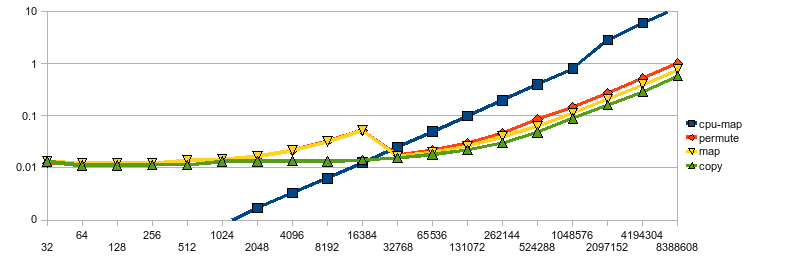
\includegraphics[width=1.0\textwidth]{bench-map.png}

Ved omkring $2^{15}$ elementer bliver vores GPGPU-implementation af map hurtigere end en
simpel CPU-version, og er mod slutningen ca. 15 gange hurtigere. 
De andre elementvise primitiver ligger tæt op af map i tidsforbrug.

\subsection{Scan}

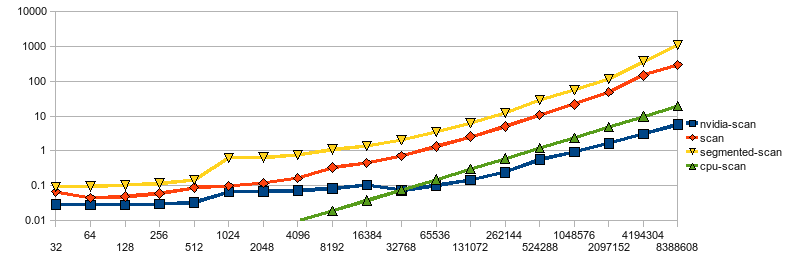
\includegraphics[width=1.0\textwidth]{bench-scan.png}

Ved omkring $2^{15}$ elementer bliver NVIDIAs GPGPU-baserede scan-implementation hurtigere 
end en simpel implementation på CPU'en.

Vores implementation af scan bliver derimod ikke hurtigere for de størrelser
vi har målt, og hvis kurven ekstrapoleres nærmer de sig heller ikke CPU-versionen. Hen mod 
slutningen af kurven er den ca. 60 gange langsommere end NVIDIAs implementation. 
Vores segmented scan er til sidst ca. fire gange langsommere end vores scan.

For store vektorer er NVIDIAs scan ca. tre gange hurtigere end CPU-versionen.

Springet på kurven for mellem 512 elementer og 1024 elementer er sandsynligvis et resultat 
af at gå fra en enkelt til to blokke, idet der som beskrevet i afsnit \ref{CUDA} kun 
kan være 512 tråde i en blok.

\subsection{Split}

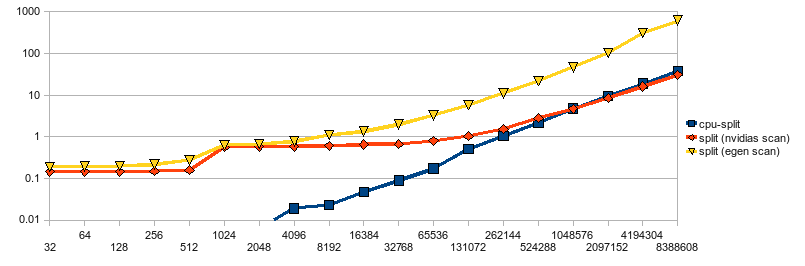
\includegraphics[width=1.0\textwidth]{bench-split.png}

Springet fra scan skinner igennem på denne kurve, da vi bruger scan i implementationen.

Det relativt mindre forhold mellem implementationen med vores scan og NVIDIAs scan kommer
af at vi udover scan også bruger de relativt hurtige elementvise primitiver.

GPGPU-versionen af split bliver aldrig markant hurtigere end den simple CPU-version,
heller ikke selvom vi anvender NVIDIAs scan.

I starten af kurven er omkostningen ved NVIDIAs scan høj, men den bliver relativt mindre
for større vektorer. NVIDIAs scan kun er tre gange hurtigere end en simpel summering på 
CPU'en (cpu-scan), og da hver iteration af cpu-radix ikke er meget mere kompleks end en
summering giver det mening at den er stort set lige så hurtig.

\subsection{Radix sort}

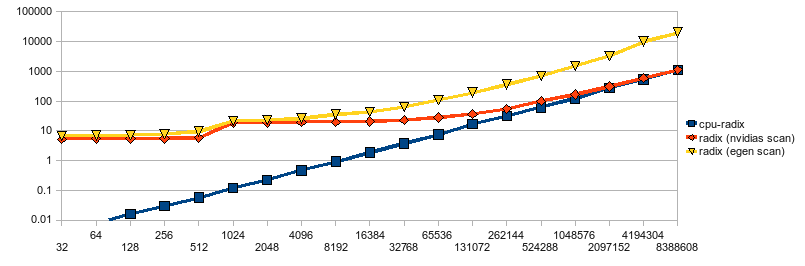
\includegraphics[width=1.0\textwidth]{bench-radix.png}

Da størstedelen af arbejdet i vores radix sort foregår i split-funktionen,
ligner kurven for de to funktioner ikke overraskende hinanden. 


% -*- coding: utf-8 -*-

% NOTER TIL DETTE AFSNIT:
% - Fokus bør være på at videregive den viden vi har opnået, og hvordan man burde gøre
%   det - de steder hvor vi har taget fejl kan bruges som kontrast.
% - Hvorfor er vores implementation langsom (referer til benchmarks og implementation).
% - Hvad burde man gøre istedet?
% - Hvor hurtigt kunne man forvente at det ville køre med disse forbedringer?
%   Lav evt. benchmark hvor der måles hvor lang tid scan tager i sorteringsalgoritmen, 
%   og sammenlign med et tilsvarende benchmark af deres scan i isolation.
% - Burde man have lavet benchmarks løbende helt fra starten, og fokuseret på hastighed
%   før API'et? Ja, for på den måde kan man tidligst muligt se om det giver mening 
%   overhovedet, og man risikerer ikke at lave et API der har et indbygget overhead.
% - For at en implementation på CUDA skal give mening skal programmet køre mange gange
%   hurtigere (ellers er det nemmere at bruge CPU'en).
%   Hvor meget arbejde kræver det at lave en sådan algoritme? For scan or sortering:
%   Linjer kode på CPU, linjer kode i hele vores implementation, linjer kode oven på
%   API'et (meget færre, gør dette til en pointe), linjer i deres implementation.
%   Derudover CUDA-specifikke hukommelsesmodeller, eksekveringsmodeller og begrænsninger.
% - Meget ``manuel'' hukommelses- og control-flow optimering.
% - Det er vigtigt at finde ud af om vector-scan-modellen giver mening på CUDA!

\section{Analyse}

\subsection{Forbedringer}

I løbet af udviklingen løb vi ofte ind i segmentation faults som følge af at
følge en pointer til hukommelse der var allokeret på grafikkortet, eller
fordi vi gav en pointer til hukommelse på værtsystemet videre til en
funktion der forventede at det lå på grafikkortet.
For at undgå dette kunne man ændre \verb|PARACUDA_*_allocate_device|
så den returnerede en \verb|device_vector_t| der ikke kunne anvendes som en
pointer af brugeren. Tilsvarende skulle \verb|PARACUDA_*_copy_device_host|
tage en \verb|device_vector_t| og en normal pointer, istedet for at tage
normale pointere som begge argumenter. Hvis man tilpassede hele biblioteket
på den måde, kunne man helt undgå de segmentation faults der er relaterede 
til hvor hukommelsen er allokeret.

Radix- og split-algoritmerne bruger midlertidige vektorer, som de allokerer
ved start og frigør i slutningen af funktionen.
Dette gav ikke nogen mærkbar omkostning i vores tilfælde fordi kroppen tog
relativt lang tid at køre. Hvis det ikke var tilfældet, kunne en måde at 
undgå det på være at lave en klasse der allokerede de midlertidige vektorer
ved oprettelse og frigjorde dem ved nedlæggelse (construction og destruction),
og så have selve funktionen som en metode.
På den måde kunne man beholde klassen i hukommelsen og undgå allokeringer
i hvert kald til funktionen.

\subsubsection*{NVIDIAs implementation af scan}

NVIDIAs scan for små vektorer er implementeret så den starter med at hente
elementer fra den globale hukommelse ind i shared memory. Alle beregninger
foretages så på shared memory hvorefter resultatet skrives tilbage i den
globale hukommelse.

De deler vektoren op i dele der passer i en blok og bruger scan for små
vektorer på hver del i hver sin blok.

Derefter laver de scan på en vektor der indeholder summen af hver blok,
og til sidst lægger de hvert af disse elementer til den tilsvarende bloks
delvektor.

Dermed opnår de maksimal samtidighed, da hvert element har sin egen tråd,
og trådene er delt ud over mange blokke så de kan køre på flere cores.

En mere udførlig beskrivelse kan findes i \cite{harris}.

\subsection{Arbejdsbyrde}

Den parallele scan-algoritme er i \cite{gpu-scan} ca. 10 linjer lang. NVIDIAs implementation
(i scanLargeArray-eksemplet i deres CUDA SDK) er ca. 500 linjer lang.
I dette eksempel er 98\% af koden altså dedikeret til C- eller CUDA-specifikke 
optimeringer eller problemer, og den kan stadig ikke håndtere vektorstørrelser på over 
$2^{24}$.

Da det altid vil være en investering at bruge en ny teknologi, og da teknologien typisk
ikke er lige så tilgængelig som konventionelle CPU'er, er det nødvendigt at en 
implementation på CUDA kører betydeligt hurtigere end en normal CPU-implementation før
det kan betale sig at benytte teknologien.
I vores benchmarks er NVIDIAs CUDA-implementation af scan for store vektorer ca. tre gange 
hurtigere end den sekventielle version, hvilket ikke nødvendigvis er nok til at gøre det
besværdet værd.

Set fra en anden vinkel, hvis dette er en indikator for hvor meget arbejde der skal lægges i 
at implementere noget på CUDA, bør man grundigt overveje hvorvidt den ekstra arbejdsbyrde er 
den potentielle hastighedsforøgelse værd.

NVIDIAs CUDA-hjemmeside har en oversigt over implementerede algoritmer på CUDA og hvor mange
gange hurtigere de kører end deres CPU-implementation. Selvom de ikke nødvendigvis er perfekte
sammenligninger, kan de give en ide om hvilke typer af algoritmer der er velegnet til CUDA og 
hvilke der ikke er.

\subsection{Vector-scan-modellen på CUDA}

NVIDIAs egen implementation af scan er begrænset til at arbejde på en vektor af 
floating point tal, men der er ingen teknisk grund til at den ikke kan generaliseres 
til  vilkårlige vektorer. Dermed kan man erstatte den underliggende implementation 
af scan i vores bibliotek med deres langt hurtigere version.

For hver tredje Scan man laver kan man lave en simpel iteration svarende til en summering 
hen over sin vektor på CPU-en, hvilket betyder at hvis man har en sekventiel algoritme med 
relativt simple iterationer (som for eksempel radixsort), kan den parallele version højest
benytte tre scans per iteration før den bliver langsommere (under antagelse af at de bruger
samme antal iterationer).

Det er svært at forestille sig tilfælde hvor en scan eller Segmented Scan der kun er tre
gange hurtigere på grafikkortet kan føre til signifikant mindre tidsforbrug.

Man skal naturligvis tage det hardware vi har målt på og vores metode i betragtning - det
er ikke åbentlyst om det er fair at sammenligne de to typer hardware. Derudover giver CUDA
mulighed for at afvikle algoritmerne på GPGPU'en mens CPU'en arbejder på noget andet, 
hvilket gør at det kan være en fordel selvom det ikke er hurtigere.

% -*- coding: utf-8 -*-

% NOTER TIL DETTE AFSNIT:
% - API design
% - For langsomt (ikke i brugbar stand, CPU hurtigere)
% - Arbejdskrævende

\section{Konklusion}

\subsection{Hastighed}
Som det klart fremgår i \ref{Benchmarks}, er vores program meget langsommere end både NVIDIAs implementation, og en tilsvarende algoritme på CPU'en. Ud fra dette bliver vi nød til at konkludere at vores implementation ikke på nuværende tidspunkt er praktisk anvendeligt, og at yderligere arbejde ville være nødvendigt for at få den til at virke tilfredstillende. Vores målinger viser dog også at Radixsort, som implementeret efter \cite{ble} ikke er interessant, da scan er for langsom (hvis man arbejder på hardware med et lignende forhold mellem sig som det vi
har målt på).

\subsubsection{Fremtidig fokus på optimeringer}
Ud fra de erfaringer vi har gjort os med NVIDIAs platform, vil vores råd være at fremtidigt arbejde vil fokusere på optimering af hukommelsen, hvilket i praksis betyder at den delte hukommelse skal udnyttes bedre og at bank conflicts skal undgås. Dette efter al sandsynlighed også betyde at der i fremtidige projektor også skal lægges vægt på at den udenomliggende kode der skal dele kaldene til kernelen op, da grafikkortet har begrænset delt hukommelse. Det er desuden klart at der i fremtidige biblioteker skal være fokus på både at håndtere data der er blevet kopieret data til GPU'en såvel som at dette ikke skal håndteres af kaldene til primitiverne.

Desuden skal man lægge vægt på at opnå maksimal samtidighed ved at fylde så mange blokke op som muligt.

\subsection{Mulighed for arbitrære operatorer}
Dog har vores projekt vist at det er muligt at skabe et bibliotek af scan primitiver som kan arbejde på arbitrært data med en abitrær operator - og at når koden først er blevet skrevet, så er det let at define nye funktioner. 

% -*- coding: utf-8 -*-

\appendix

\section{Data for tidsforbrug}
\label{benchmark-data}

Første række er antal elementer og første søjle er navne på de kørte funktioner.
Tidsforbruget er opgivet i millisekunder.
\\\\
{\scriptsize
\begin{tabular}{lrrrrrrrrrrrrrrrrrrr}
&32&64&128&256&512&1024&2048&4096&8192&16384\\
nvidia-scan&0.03&0.03&0.03&0.03&0.03&0.06&0.07&0.07&0.08&0.11\\
cpu-radix&0&0.01&0.02&0.03&0.06&0.12&0.23&0.47&0.91&1.85\\
cpu-split&0&0&0&0&0&0&0.01&0.01&0.02&0.05\\
cpu-map&0&0&0&0&0&0&0&0&0.01&0.01\\
cpu-scan&0&0&0&0&0&0&0&0.01&0.02&0.04\\
scan&0.07&0.04&0.05&0.06&0.09&0.1&0.12&0.17&0.33&0.45\\
segmented-scan&0.09&0.09&0.1&0.12&0.15&0.62&0.65&0.75&1.09&1.4\\
permute&0.01&0.01&0.01&0.01&0.01&0.01&0.02&0.02&0.03&0.05\\
map&0.01&0.01&0.01&0.01&0.01&0.01&0.02&0.02&0.03&0.05\\
copy&0.01&0.01&0.01&0.01&0.01&0.01&0.01&0.01&0.01&0.01\\
split&0.19&0.19&0.2&0.22&0.27&0.64&0.68&0.77&1.1&1.34\\
radix&6.66&6.84&7.14&7.68&9.52&21.38&22.55&25.56&35.64&42.87\\
nvidia-split&0.14&0.14&0.14&0.15&0.16&0.57&0.57&0.58&0.6&0.65\\
nvidia-radix&5.25&5.31&5.35&5.49&5.76&18.97&19.04&19.38&19.67&20.75\\
\end{tabular}}
\\\\
{\scriptsize
\begin{tabular}{lrrrrrrrrrrrrrrrrrrr}
&32768&65536&131072&262144&524288&1048576&2097152&4194304&8388608&\\
nvidia-scan&0.07&0.1&0.15&0.24&0.56&0.93&1.65&3.03&5.75&\\
cpu-radix&3.72&7.39&16.58&31.56&61.42&122.36&269.17&537.05&1081.44&\\
cpu-split&0.09&0.17&0.5&1&2.08&4.77&10.02&19.12&40.17&\\
cpu-map&0.03&0.05&0.1&0.2&0.47&0.81&2.75&6.03&12.36&\\
cpu-scan&0.07&0.15&0.3&0.59&1.19&2.37&4.77&10.2&20.4&\\
scan&0.72&1.34&2.56&5&10.9&21.66&48.79&149.02&297.98&\\
segmented-scan&2.04&3.47&6.33&12.19&29.35&56.79&116.53&369.59&1127.52&\\
permute&0.02&0.02&0.03&0.05&0.09&0.15&0.28&0.53&1.02&\\
map&0.02&0.02&0.03&0.04&0.07&0.12&0.21&0.4&0.77&\\
copy&0.02&0.02&0.02&0.03&0.05&0.09&0.16&0.32&0.56&\\
split&1.95&3.26&5.85&11.01&21.74&46.12&102.95&308.3&615.38&\\
radix&64.41&106.5&190.81&358.25&695.45&1496.3&3329.77&9938.08&19847.44&\\
nvidia-split&0.66&0.79&1.03&1.51&2.78&4.67&8.44&16.09&30.8&\\
nvidia-radix&22.88&27.69&36.16&54.08&98.1&166.83&305.31&583.72&1127.22&\\
\end{tabular}}

\section{Kildekode}

\sourcecode{main.cpp}{code-main}{main.cpp}
\sourcecode{test.cu}{code-test}{test.cu}
\sourcecode{kernel.cu}{code-kernel}{kernel.cu}
\sourcecode{copy.h}{code-copy}{copy.h}
\sourcecode{split.h}{code-split}{split.h}
\sourcecode{radix.h}{code-radix}{radix.h}
\sourcecode{arrayprint.h}{code-arrayprint}{arrayprint.h}
\sourcecode{paracuda.h}{code-paracuda}{paracuda.h}
\sourcecode{paracuda_struct.h}{code-struct}{paracuda\_struct.h}
\sourcecode{paracuda_map.h}{code-map}{paracuda\_map.h}
\sourcecode{paracuda_permute.h}{code-permute}{paracuda\_permute.h}
\sourcecode{paracuda_scan.h}{code-scan}{paracuda\_scan.h}
\sourcecode{paracuda_segmentedScan.h}{code-segmented-scan}{paracuda\_segmentedScan.h}
\sourcecode{nvidia_scan.h}{code-nvidia-scan}{nvidia\_scan.h}
\sourcecode{nvidia_kernel.cu}{code-nvidia-kernel}{nvidia\_kernel.cu}
\sourcecode{nvidia_large_kernel.cu}{code-nvidia-large-kernel}{nvidia\_large\_kernel.cu}
\sourcecode{cpu_map.h}{code-cpu-map}{cpu\_map.h}
\sourcecode{cpu_scan.h}{code-cpu-scan}{cpu\_scan.h}
\sourcecode{cpu_split.h}{code-cpu-split}{cpu\_split.h}
\sourcecode{cpu_radix.h}{code-cpu-radix}{cpu\_radix.h}


% -*- coding: utf-8 -*-

\begin{thebibliography}{99}

\bibitem[Blelloch]{ble} Guy E. Blelloch, \emph{Vector Models for Data-Parallel Computing}, 1990.

\bibitem[Harris]{harris} M Harris, \emph{Parallel Prefix Sum (Scan) with CUDA}, available at
\url{http://developer.download.nvidia.com/compute/cuda/sdk/website/projects/scan/doc/scan.pdf}, January 2008.

\bibitem[Shubhabrata]{gpu-scan} Sengupta, Harris, Zhang and Owens, \emph{Scan primitives for GPU computing}, available at
\url{http://www.idav.ucdavis.edu/func/return_pdf?pub_id=915}, April 2001.

\bibitem[Guide]{cuda-guide} NVIDIA, \emph{CUDA 2.1 Programming Guide}, available at
\url{http://www.nvidia.com/object/cuda_develop.html}, November 2008

% husk cuda-model

\hide{
@inproceedings{1280110,
 author = {Sengupta,, Shubhabrata and Harris,, Mark and Zhang,, Yao and Owens,, John D.},
 title = {Scan primitives for GPU computing},
 booktitle = {GH '07: Proceedings of the 22nd ACM SIGGRAPH/EUROGRAPHICS symposium on Graphics hardware},
 year = {2007},
 isbn = {978-1-59593-625-7},
 pages = {97--106},
 location = {San Diego, California},
 publisher = {Eurographics Association},
 address = {Aire-la-Ville, Switzerland, Switzerland},
 }

}

\end{thebibliography}

\end{document}

